\titleformat{\chapter}[hang]{\linespread{1}\heiti\sanhao\bfseries\filright}{\thechapter}{1em}{}{}
\renewcommand*{\thefigure}{\arabic{figure}}
\chapter{模型评估}
为了更直观地展示不同去噪模型的效果,我采用Python来加载图像,并实现了ROF(Rudin-Osher-Fatemi)模型和LLT(Low-Latency Trendline)模型。通过Matplotlib库进行可视化,我们可以进行benchmark比较,以评估这些模型在去除噪声方面的性能。(代码位于\href{https://github.com/mysciz/MPE}{Github})

\section{ROF模型}
我们首先通过合成噪声图像对ROF模型进行检验,我们利用噪声创建一个500x500的图像矩阵,并分别对他进行ROF去噪和高斯滤波,得到以下结果。
\vspace{-1em}
\begin{figure}[h]
    \centering
    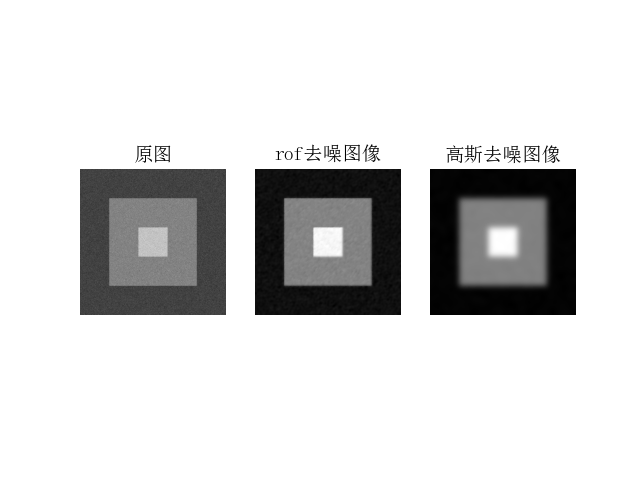
\includegraphics[width=0.8\textwidth]{Images/合成评估.png}
    \vspace{-7em}
    \caption{合成评估}
    \label{fig:synthesis_evaluation}
\end{figure}
我们可以看出原始图像显示为较暗的灰色正方形,ROF去噪图像则显示为白色正方形,通过Rudin-Osher-Fatemi模型处理后,图像变得更加明亮和清晰,有效减少噪声同时保留重要特征。高斯去噪图像也显示为白色正方形,通过高斯函数减少高频噪声,图像更加平滑。

之后我们对实际图像进行相同的处理。
\begin{figure}[ht]
    \centering
    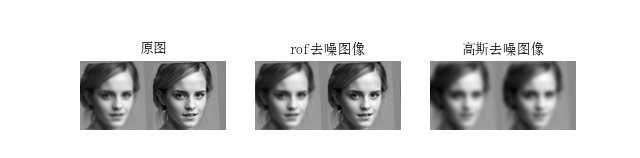
\includegraphics[width=1\textwidth]{Images/real.png}
    \vspace{-2em}
    \caption{实例评估}
    \label{fig:synthesis_evaluation}
\end{figure}
\FloatBarrier

从图像中我们可以看出,ROF模型可以保留原图像大趋势部分,使图像变得更加明亮和清晰,而高斯去噪将图像更加平滑,但也导致了图像变得更加模糊,从而导致不好的效果。

从上述比较可以看出,相较于高斯滤波,ROF模型具有更高的收敛性、稳定性。实际上,ROF模型解的存在是唯一的,这为模型的稳定性和可靠性提供了理论保障。\cite{rudin1994total}ROF模型不仅适用于去除高斯噪声和泊松噪声,还可以应用于其他类型的图像去噪任务中,具有广泛的应用前景。

\section{LLT模型}
同样,对比TV模型、LLT模型和改进的LLT模型的图像恢复效果.采用256×256像素的“Lena”图像
作为测试图像,如图3所示
\begin{figure}[ht]
    \centering
    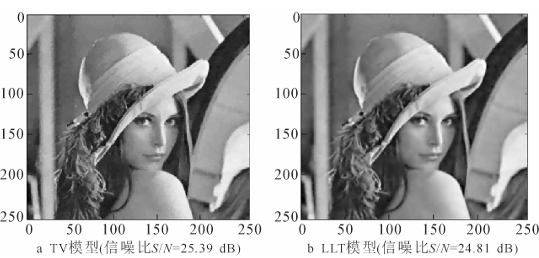
\includegraphics[width=0.5\textwidth]{Images/lena.png}
    \vspace{-1em}
    \caption{lena\cite{JSDN201705008}}
    \label{fig:synthesis_evaluation}
\end{figure}
\FloatBarrier
可以看出,LLT模型对图像光滑部分的恢复效果很好,但是在一定程度上模糊了图像的边缘。